\section{\methodNameGeneral - a Multiobjective Evolutionary Approach}

\subsection{Architectural Overview}
\label{sec:method-overview}

The proposed layout generation method, coined \methodNameGeneralLong (\methodNameGeneral), is engineered as a multi-objective evolutionary framework that find a set of layouts $\solution$ for a given instance $\instance$ of the above-detailed problem.  

\begin{figure}[h]
    \centering
    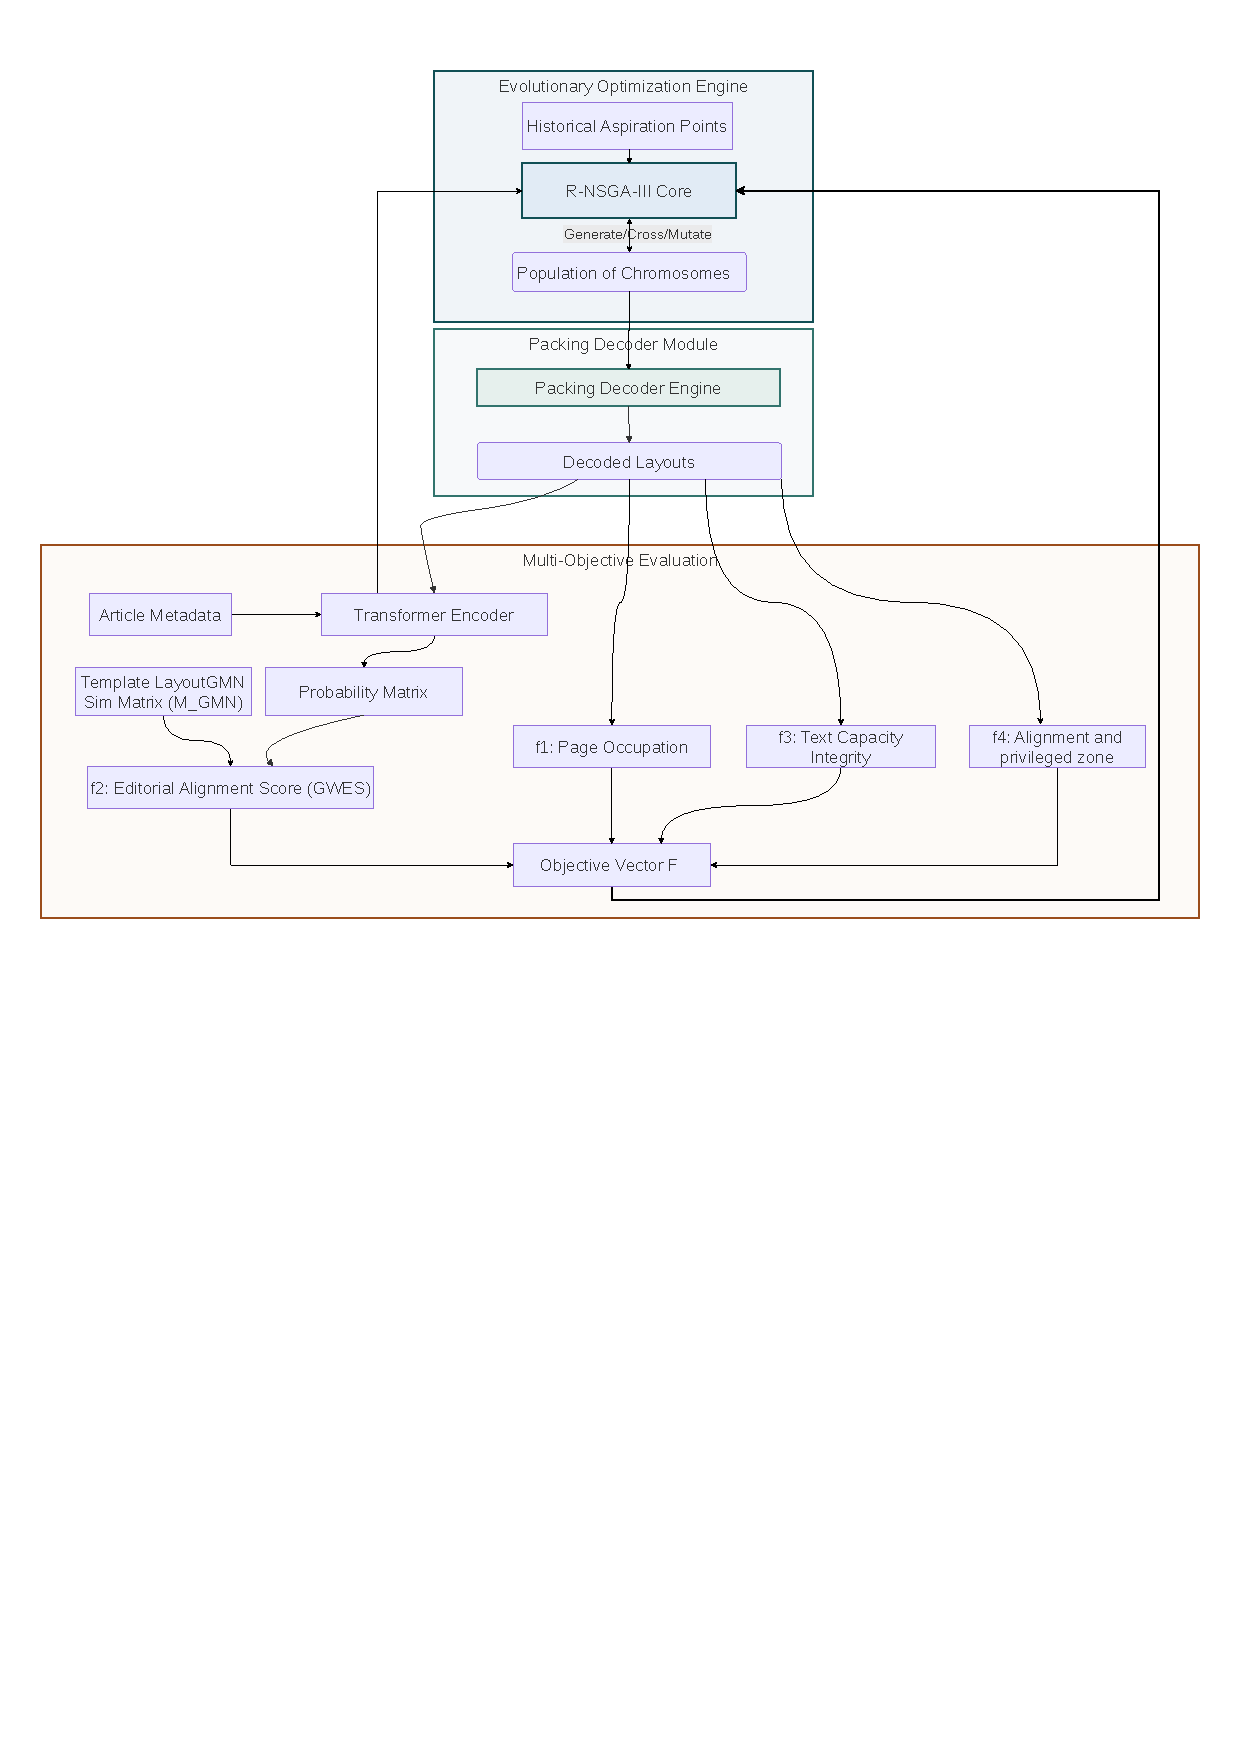
\includegraphics[width=\widthForOneImage]{img/method/method-overview.pdf}
    \caption{Global architectural workflow of the proposed \methodNameGeneral\ framework. }
    \label{fig:method-overview}
\end{figure}

The global workflow of \methodNameGeneral operates as an optimization pipeline structured across three main interconnected modules, as illustrated in Figure~\ref{fig:method-overview}. 

\begin{itemize}
    \item \textbf{Many-Objective Evolutionary Optimization Engine:} Operating as the strategic search core, this module manages the population of abstract chromosomes across generations through specialized genetic operators (crossover, mutation, and pareto-front based selection~\cite{pareto}). The engine navigates the combinatorial search space of chromosomes, which represents template assignments ($\templatesel{i}$), article positioning $\posvar{i}$, and vertical elasticities $\elasticity{i}$.  Additionally, this module implements two distinct paradigms to select the best chromosomes in each generation: a preference-guided RNSGA-III~\cite{rnsga-iii}, coined \methodName, which injects historical human design preferences as multi-dimensional aspiration points to drive convergence toward high-utility regions of the search space, or a standard uniform NSGA-III~\cite{nsga-iii-pt1, nsga-iii-pt2}, coined \methodNameUniform, for unconstrained Pareto front that uses standard Das-Dennis~\cite{das-dennis} reference directions.

    \item \textbf{Packing Decoder Module:} Acting as the layout decoder, this module translates abstract chromosome representations into concrete layouts $\solution$ on the page canvas $\page$. By coupling the evolutionary permutation sequence with an extreme-points backtracking routine~\cite{crainic-extreme-points}, the decoder physically positions each article block while strictly guaranteeing zero spatial overlaps and enforcing sheet margin boundaries. It is important to note that while a faster and greedy heuristic could be used for this task~\cite{lodi-packing-survey, chazelle-bl, burke-bf}, resolving the layout(i.e., resolving each decision variable in Chapter~\ref{sec:decision-variables}, conditioned to the specifications fixed by the abstract chromosome) remains computationally tractable, given that instances consistently involve a small number of articles ($\numarticles < 9$). This property allows the use of exact backtracking routines such as extreme-points method~\cite{crainic-extreme-points}.

    \item \textbf{Multi-Objective Evaluation Module:} This module dynamically assesses each decoded layout $\solution$ across the four-dimensional objective space to synthesize the unified objective vector $\objvector(\solution)$. It combines analytical geometric functions ($\objone$: Page coverage, $\objthree$: Text capacity Integrity, and $\objfour$: Positioning of articles quality) with a neural evaluation pipeline ($\objtwo$: \NeuralMethod). The resulting objective vector  $\objvector(\solution)$ is fed back into the evolutionary optimization module to drive chromosome selection in the next generation.
\end{itemize}


\subsection{Multi-Objective NSGA-III Optimization Engine}
\label{sec:evolutionary_engine}

The evolutionary engine optimizes layout configurations across the four-dimensional objective space defined in Chapter~\ref{sec:objective_formulation}. To navigate this search space, each candidate solution $\solution$ is encoded as a chromosome vector that maps abstract decisions prior to layout decoding using the packing engine.


%%%% Chromosome Representation %%%
\subsubsection{Chromosome Representation}
\label{sec:chromosome_representation}

Each candidate layout $\solution$ is encoded as a chromosome composes of three sub-vectors $\chromosome = \langle \chromosomeTemplateSegment, \chromosomePermutationSegment, \chromosomeElasticitySegment \rangle$ that captures the  design choices for the $\numarticles$ active articles, as illustrated in \figref{fig:chromosome_representation}:

\begin{enumerate}
    \item \textbf{Template Assignment Segment} $\chromosomeTemplateSegment = [t_1, t_2, \dots, t_{\numarticles}]$: A vector where each gene $t_i \in \{1, \dots, \catalogsize\}$ defines the specific template assigned to article $\articleobj{i}$ from \templatecatalog.
    \item \textbf{Permutation Segment} $\chromosomePermutationSegment = [\pi_1, \pi_2, \dots, \pi_{\numarticles}]$: A vector representing a permutation of the default input article indices $\{1, 2, \dots, \numarticles\}$. This segment explicitly dictates the sequence in which the packing decoder engine must process and position each article on the page.
    \item \textbf{Text Elasticity Segment} $\chromosomeElasticitySegment = [e_1, e_2, \dots, e_{\numarticles}]$: A vector where each gene $e_i \in \elasticityset$, defining the specific vertical elasticity (see Chapter~\ref{sec:decision-variables}).
\end{enumerate}


\begin{figure}[htbp]
    \centering
    \begin{tikzpicture}[
        box/.style={draw, minimum size=8mm, inner sep=0pt, font=\small},
        idx/.style={font=\small, text=gray},
        sublabel/.style={font=\small\bfseries}
    ]

    % Main chromosome label on the left
    \node[font=\small\bfseries] (chrom-label) at (-0.8, 0) {$\chromosome = $};

    % --- 1. Template Segment (\chromosomeTemplateSegment) ---
    \node[box] (t1) at (0,0) {4};
    \node[box, right=-\pgflinewidth of t1] (t2) {12};
    \node[box, right=-\pgflinewidth of t2] (t3) {1};
    \node[box, right=-\pgflinewidth of t3] (t4) {7};

    % Article indices i above template segment
    \node[idx, above=2mm of t1] {$1$};
    \node[idx, above=2mm of t2] {$2$};
    \node[idx, above=2mm of t3] {$3$};
    \node[idx, above=2mm of t4] {$4$};
    %\node[idx, left=2mm of idx-1, font=\small\bfseries, text=gray] {$i$:};

    % --- 2. Permutation Segment (\chromosomePermutationSegment) ---
    % Separated by a 5mm horizontal gap; NO indices placed above
    \node[box, right=2mm of t4] (p1) {2};
    \node[box, right=-\pgflinewidth of p1] (p2) {4};
    \node[box, right=-\pgflinewidth of p2] (p3) {1};
    \node[box, right=-\pgflinewidth of p3] (p4) {3};

    % --- 3. Elasticity Segment (\chromosomeElasticitySegment) ---
    % Separated by a 5mm horizontal gap
    \node[box, right=2mm of p4] (e1) {0};
    \node[box, right=-\pgflinewidth of e1] (e2) {-5};
    \node[box, right=-\pgflinewidth of e2] (e3) {10};
    \node[box, right=-\pgflinewidth of e3] (e4) {0};

    % Article indices i above elasticity segment
    \node[idx, above=2mm of e1] {$1$};
    \node[idx, above=2mm of e2] {$2$};
    \node[idx, above=2mm of e3] {$3$};
    \node[idx, above=2mm of e4] {$4$};

    % --- Bottom Grouping Braces & Sub-array Labels ---
    \draw[decorate, decoration={brace, mirror, amplitude=4pt}] 
        ([yshift=-2mm]t1.south west) -- ([yshift=-2mm]t4.south east)
        node[midway, below=5pt, sublabel] {$\chromosomeTemplateSegment$};

    \draw[decorate, decoration={brace, mirror, amplitude=4pt}] 
        ([yshift=-2mm]p1.south west) -- ([yshift=-2mm]p4.south east)
        node[midway, below=5pt, sublabel] {$\chromosomePermutationSegment$};

    \draw[decorate, decoration={brace, mirror, amplitude=4pt}] 
        ([yshift=-2mm]e1.south west) -- ([yshift=-2mm]e4.south east)
        node[midway, below=5pt, sublabel] {$\chromosomeElasticitySegment$};

\end{tikzpicture}

\caption{Chromosome representation example for an instance with $\numarticles=4$ active articles. The chromosome vector $\chromosome = \langle \chromosomeTemplateSegment, \chromosomePermutationSegment, \chromosomeElasticitySegment \rangle$ groups abstract choices for a single solution $\solution$. For the template sub-vector $\chromosomeTemplateSegment$ and the text elasticity sub-vector $\chromosomeElasticitySegment$, the index $i$ maps directly to article $a_i$, specifying its assigned template $\templatesel{i}$ and elasticity $\elasticity{i}$, respectively. Conversely, the permutation segment $\chromosomePermutationSegment$ establishes the processing sequence to build the layout; in this representative example, the packing decoder sequentially accommodates article $\articleobj{2}$, followed by $\articleobj{4}$, $\articleobj{1}$, and finally $\articleobj{3}$.}
\label{fig:chromosome_representation}
\end{figure}

%%%%%% Operators %%%%%%%%

\subsubsection{Evolutionary Operators}
\label{sec:evolutionary_operators}

To effectively manipulate the three distinct genetic components within the chromosome $\chromosome = \langle \chromosomeTemplateSegment, \chromosomePermutationSegment, \chromosomeElasticitySegment \rangle$, specialized initialization, crossover, and mutation mechanisms are implemented.

\paragraph{Population Initialization}

Given the vast combinatorial search space and strict constraints, purely random sampling populates early generations with unpromising or bad-quality candidates. Instead, a targeted initialization strategy biases the search toward feasible configurations. 

Accordingly, the initial population is structured across the chromosome segments as follows:
\begin{itemize}
    \item \textbf{\chromosomeTemplateSegment:} 50\% of the individuals are sampled using baseline \neuralmethod\ probabilities. Since no geometric layout exists at generation zero, this initial query feeds the Transformer with a \emph{metadata-only tensor}, where spatial coordinates and template zoning are omitted. Due to its training with feature dropout, the model is inherently robust to this missing spatial context, successfully projecting a meaningful predictive distribution that guides the initial sampling away from random choices. Of the remaining population, 30\% are sampled uniformly from a feasible template subset that satisfies all hard constraints and yields zero text capacity penalty ($\objthree = 0$). The final 20\% are randomized from a subset that satisfies all hard constraints. 

    \item \textbf{\chromosomePermutationSegment: } Individuals are initialized by generating uniform random permutations of article's sequence $\{1, 2, \dots, \numarticles\}$.  This initialization generates valid permutations of article indices rather than independent random integers, strictly guaranteeing that every article receives a unique sequence index without duplicates or missing elements.

    \item \textbf{\chromosomeElasticitySegment: } The majority of the initial population (80\%) is initialized with null vertical elasticity ($\elasticity{i} = 0$), establishing an uncompressed state across initial solutions. However, the remaining 20\% is initialized with stochastically sampled elasticity values $\elasticity{i} \in \elasticityset$. This controlled injection of elasticity variance allows the evolutionary search to explore compression and expansion trade-offs from the beginning.
\end{itemize}



\paragraph{Crossover}

The crossover operator applies two concurrent strategies, to account for the different nature of the chromosome segments:

\begin{itemize}
    \item \textbf{$\chromosomeTemplateSegment$} and \textbf{$\chromosomeElasticitySegment$} segments: standard Two-Point Crossover~\cite{crossovers} is executed.
    \item \textbf{$\chromosomePermutationSegment: $} to maintain valid indexing constraints without duplicates in the permutation sequence, the permutation segment ($\chromosomePermutationSegment$) is crossed using Order Crossover (OX1)~\cite{crossovers}.
\end{itemize}

\begin{figure}[htbp]
    \centering
    %%

    \caption{Two-point crossover}
\end{figure}
\begin{figure}[htbp]
    \centering
    %%

    \caption{Order Crossover (OX1)}
\end{figure}


\paragraph{Mutation Roulette}

To navigate the search space defined by the chromosome, a single uniform mutation operator is insufficient. Because the chromosome simultaneously encodes three distinct decision variables, each variable type requires specialized structural manipulation. A multi-operator mutation strategy is therefore designed,
where each mutation operator is managed by a hierarchical orchestrator. A global mutation probability $\globalmutationprob$ determines whether an individual undergoes modification. If triggered, exactly one specialized mutation operator is selected via a stochastic roulette wheel governed by a weight vector $\mathbf{w} = [\mutationprob{1}, \mutationprob{2}, \mutationprob{3}, \mutationprob{4}, \mutationprob{5}, \mutationprob{6}]$, where $\sum_{m=1}^{6} \mutationprob{m} = 1$. This design balances fine-grained local search, targeted constraint repair, and broad global exploration across all variables represented in the chromosome.

The six specialized mutation operators are defined as follows:

\begin{itemize}
    \item \textbf{Permutation Reverse} ($\mutationprob{1}$): Selects a random sub-sequence within the permutation segment $\boldsymbol{\pi}$ and reverses its order, altering the priority sequence passed to the packing engine.
    \item \textbf{5-Most Similar Template} ($\mutationprob{2}$): Selects a random article and queries the matrix $\gmnMatrix$ to extract its $K=5$ topologically closest template neighbors. A new template is stochastically sampled from this neighborhood based on their  \neuralmethod\ scores (metadata-only tensor).
    \item \textbf{Textual Integrity Improvement} ($\mutationprob{3}$): Evaluates the current layout to identify the specific article causing the worst local capacity violation within objective $\objthree$. It then aggregates a feasible pool of templates that satisfy the article's physical requirements ($\objthree \sim 0$), replacing the mismatched template with a randomly selected  alternative from this pool.
    \item \textbf{Bernoulli Template Resampling} ($\mutationprob{4}$): Executes an independent Bernoulli trial with success probability equal to $0.5$ for every gene in the template segment $\chromosomeTemplateSegment$. For each winning gene, a new template is re-sampled globally from the entire catalog following the \neuralmethod probability distribution.
    \item \textbf{Random Template Substitution} ($\mutationprob{5}$): Replaces a randomly selected article's template with a completely random choice from the catalog boundaries, injecting pure structural exploration.
    \item \textbf{Geometric Elasticity Adjustment} ($\mutationprob{6}$): Selects a random gene from the elasticity segment $\chromosomeElasticitySegment$ and applies a fine-tuning delta ($\pm 5$). The mutated value is automatically clipped to remain within the operational boundaries of $[-15, 15]$.
\end{itemize}

Crucially, to preserve context, whenever a $\chromosomeTemplateSegment$ mutation ($\mutationprob{2}, \mutationprob{3}, \mutationprob{4}, \mutationprob{5}$) modifies an article's template assignment, its corresponding elasticity gene in $\chromosomeElasticitySegment$ is automatically reset to 0.


%%%%%% NSGA specifics %%%%%%%%%%

\subsubsection{Many-Objective Optimization Paradigm}
\label{sec:many-objective_optimization}

The evolutionary optimization process runs for $\ngen$ generations over the objective space defined in Chapter~\ref{sec:objective_formulation}. To incorporate domain expertise, \methodNameGeneral\ implements two variants for the multi-objective selection: a targeted aspiration-point design (\methodName) as a preference-based method, and a uniform exploratory variant (\methodNameUniform).

\paragraph{Preference-Guided Engine (\methodName)}
To actively guide the evolutionary search toward layout configurations adhering to real-world publishing standards, the first configuration of the proposed method, coined \methodNameLong\ (\methodName), instantiates a Reference-Point NSGA-III (RNSGA-III) paradigm~\cite{rnsga-iii}. Instead of allowing the population to disperse across regions that, while mathematically non-dominated, deviate from established industry standards, the search is explicitly directed by historical aspiration vectors. These reference coordinates are computed offline from the objective vector distributions observed within the historical training dataset (see \secref{subsec:dataset_characterization}), conditioned on the active article count $\numarticles$ of the instance \instance. Specifically, for the four-dimensional objective space distribution of historical layout designs, two distinct aspiration vectors are extracted, corresponding to the 25th percentile (first quartile) and the 50th percentile (median) of the empirical historical distributions. Because all objectives follow a minimization paradigm, these quantiles establish demanding yet realistic target thresholds derived directly from successful human designs. A radius parameter $\RNSGAradius$ is enforced around these targeted points, restricting exploration to regions of proven structural and editorial utility. 

To preserve localized diversity within these two targeted points, the framework projects a structured set of reference directions around each aspiration vector using 8 partitions, which mathematically yields exactly 165 local directions for a 4-dimensional space~\cite{rnsga-iii}. Accordingly, we configure a population size of 165 individuals per reference point ($165 \times 2 = 330$ in total), satisfying the preference-guided mechanism requirements while maintaining an equitable search capacity relative to the uniform exploration baseline.



%TODO THIS REQUIRES MORE EXPLANATION


\paragraph{Uniform Exploration (\methodNameUniform)}

To ensure an unbiased and wide-reaching exploration of the non-dominated multi-objective frontier, the second variant, coined \methodNameUniformLong\ (\methodNameUniform) uses standard NSGA-III~\cite{nsga-iii-pt1, nsga-iii-pt2}. This variant  operates fully autonomously without requiring historical design aspiration points, making it uniquely valuable when explicit editorial guidelines are unavailable or when the relative priorities among objectives are completely unknown. Reference directions are systematically generated via the Das-Dennis method~\cite{das-dennis} using 10 partitions (corresponding to $\popsize = 286$ individuals), establishing a uniform mesh across the entire Pareto front. By definition, this configuration maximizes objective space coverage, providing a robust, unconstrained search space coverage that facilitates standardized mathematical benchmarks against other baselines.

%TODO This might require more explanation


%%%%%%%% Backtracking packing engine %%%%%%%%

\subsection{Packing Decoder Engine}
\label{sec:packing_engine}

The packing decoder engine is implemented to ensure a deterministic decoding of the abstract chromosome $\chromosome = \langle \chromosomeTemplateSegment, \chromosomePermutationSegment, \chromosomeElasticitySegment \rangle$ into a page layout represented by spatial coordinates and the previously defined decision variables (Chapter~\ref{sec:decision-variables}). Unlike standard two-dimensional bin packing algorithms that allow arbitrary item reordering~\cite{lodi-packing-survey, chazelle-bl, burke-bf}, this engine enforces strict sequence preservation dictated by the evolutionary permutation segment $\chromosomePermutationSegment$. 

This sequence preservation is fundamental to the multi-objective nature of the optimization problem, since changing the relative order of articles directly alters $\objvector$, meaning that different permutation sequences yield distinct non-dominated trade-offs across the multi-objective Pareto frontier. 
On the contrary, once a specific sequence $\chromosomePermutationSegment$ is fixed by the evolutionary operators, the packing engine's sole responsibility is to evaluate its geometric feasibility. By coupling a fixed linear sequence with a complete, exhaustive backtracking technique, the decoder guarantees that if a valid spatial configuration exists for that specific permutation, it will be found.

\subsubsection{Dimensions Definition}
Before triggering the packing routine, the engine maps the active chromosome genes into  physical attributes for each article $\articleobj{i}$. The template gene $\templatesel{i} \in \chromosomeTemplateSegment$ fixes the width $\Wtemp{\templatesel{i}}$ of the article based on its template assignment $\templatesel{i}$ in the catalog $\templatecatalog$. Concurrently, the discrete text elasticity step $\elasticity{i}$ is retrieved from $\chromosomeElasticitySegment$ to compute the effectively scaled height $\Hscaled{\templatesel{i}}$ that the engine will attempt to allocate, as described in Equation~\ref{eq:h-scaled}:

\begin{equation}
\Hscaled{\templatesel{i}} = \Htemp{\templatesel{i}} \cdot \left(1 + \frac{\elasticity{i}}{100}\right)
\tag{\ref{eq:h-scaled}}
\end{equation}

\subsubsection{Extreme Points-based Packing Engine}

Spatial allocation inside the page canvas builds upon the foundational Extreme Points (EPs) paradigm introduced by Crainic et al.~\cite{crainic-extreme-points}. In its standard formulation, when a rectangular item is packed, new insertion candidates are generated by projecting its top and right coordinates along the orthogonal axes until they intersect either the boundaries of an adjacent item or the container walls.

First, the list of available Extreme Points $\extremepointset$ is initially seeded with the page origin $\extremepointset = \{(0,0)\}$. 

To maintain a valid and compact search space, the candidate point list $\extremepointset$ is continuously pruned by eliminating coordinates that fall outside the page bounds $(\Weff, \Heff)$ or land inside already allocated articles. The remaining valid points within $\extremepointset$ are sorted following a canonical Bottom-Left priority sequence: any generic candidate point $P = (x_P, y_P) \in \extremepointset$ is ordered ascending by its vertical coordinate $y_P$, breaking ties by its horizontal coordinate $x_P$.

While the previous formulation corresponds to the standard approach proposed by Crainic et al.~\cite{crainic-extreme-points}, in \methodName, this step needs to be adapted to consider the grid imposed by $\colsize$ and $\gutter$. This is already taken into account by the template dimensions (as mentioned in \secref{sec:template-definition}), but is also necessary that the packing decoder engine introduces a localized alignment shift during point generation to respect the $\gutter$. Specifically, when an article $\articleobj{i}$ is successfully committed to an x-coordinate $\xcoord{i}$, the baseline extreme points are shifted by the $\gutter$ offset:
\begin{equation}
\xcoorgutter{i} = (\xcoord{i} + \Wtemp{\templatesel{i}} + \gutter, y)
\end{equation}




\subsubsection{Sequence-Preserving Backtracking Packing}


The packing engine strictly enforces the sequential order dictated by the evolutionary permutation segment $\chromosomePermutationSegment$. Considering this, the packing decoder engine processes the sequence through a dynamic prefix-slicing mechanism, as formalized in Algorithm~\ref{alg:packing_decoder}. At any point during execution, a tracking index divides the permutation into already packed items and a sub-sequence of remaining unplaced articles. The engine's objective is to isolate and accommodate the largest possible continuous block/prefix of these remaining articles in the page canvas, starting exactly from the tracking index. Crucially, maximizing this prefix size directly minimizes empty or unallocated remnants on the page canvas, thereby significantly optimizing the wasted space objective ($\objone$).


To determine if a targeted prefix can fit within the current page, the engine invokes an exhaustive recursive backtracking solver, structured in Algorithm~\ref{alg:solve_recursive}. For a given batch, the solver processes the articles sequentially, evaluating them against the sorted extreme points list $\extremepointset$. It attempts to position the current item on the first available candidate point; if the item respects the page boundaries and yields zero spatial overlap, the placement is provisionally committed. The extreme points list $\extremepointset$ is then updated, and the solver recursively calls itself to place the next article in the batch. If a downstream article cannot be accommodated on any valid point, the routine backtracks, uncommitting the immediate predecessor to explore alternative spatial configurations across $\extremepointset$. If the solver exhaustively explores all combinations and returns a global failure for that prefix, the outer loop decrementally reduces the batch size by one article and re-tests this smaller prefix on the same page, as outlined in Algorithm~\ref{alg:packing_decoder}. This decremental reduction repeats until a viable prefix successfully converges. Once a batch is committed, if there are still remaining unplaced items left in $\chromosomePermutationSegment$, the engine instantiates a new empty page, updates the tracking index, and restarts the cycle.

Crucially, the total number of pages is simply reported as an output of the decoding phase; the responsibility of enforcing the hard constraints and discarding or penalizing the solution for exceeding the single-page limit rests exclusively with the evolutionary optimization engine. Also, this recursive mechanism remains computationally tractable in practice because the linear $\mathcal{O}(n)$ extreme-point update sequence operates over a strictly bounded number of articles per page ($n < 9$ within the operational editorial domain).




\begin{algorithm}[h]
\caption{Sequence-Preserving Prefix Packing Decoder}
\label{alg:packing_decoder}
\begin{algorithmic}[1]
\REQUIRE Evolutionary chromosome segments $\chromosomePermutationSegment$ and $\chromosomeElasticitySegment$, page bounds $(\Weff, \Heff)$, and offsets $(\gutter{x}, \gutter{y})$.
\ENSURE Layout $\mathcal{S}$ and final $\text{page\_count}$.

\STATE $\text{tracking\_index} \leftarrow 1$
\STATE $\text{page\_count} \leftarrow 0$
\STATE $\mathcal{S} \leftarrow \emptyset$

\WHILE{$\text{tracking\_index} \le |\chromosomePermutationSegment|$}
    \STATE $\text{batch\_size} \leftarrow |\chromosomePermutationSegment| - \text{tracking\_index} + 1$
    \STATE $\text{success} \leftarrow \text{FALSE}$
    
    \WHILE{$\text{batch\_size} > 0$ \AND \NOT $\text{success}$}
        \STATE $\text{batch} \leftarrow \chromosomePermutationSegment[\text{tracking\_index} \dots \text{tracking\_index} + \text{batch\_size} - 1]$
        \STATE $\extremepointset \leftarrow \{(0,0)\}$ \COMMENT{Page origin}
        \STATE $\text{page\_layout} \leftarrow \emptyset$
        
        \STATE $\text{success} \leftarrow \textsc{SolveRecursive}(1, \text{batch}, \text{page\_layout}, \extremepointset, \text{page\_count})$
        
        \IF{$\text{success}$}
            \STATE $\mathcal{S} \leftarrow \mathcal{S} \cup \text{page\_layout}$
            \STATE $\text{tracking\_index} \leftarrow \text{tracking\_index} + \text{batch\_size}$
            \STATE $\text{page\_count} \leftarrow \text{page\_count} + 1$
        \ELSE
            \STATE $\text{batch\_size} \leftarrow \text{batch\_size} - 1$
        \ENDIF
    \ENDWHILE
    
    \IF{\NOT $\text{success}$ \AND $\text{batch\_size} = 0$}
        \STATE \RETURN $\text{FAILURE}$ \COMMENT{Single isolated article violates spatial bounds}
    \ENDIF
\ENDWHILE
\RETURN $\mathcal{S}, \text{page\_count}$
\end{algorithmic}
\end{algorithm}

\begin{algorithm}[h]
\caption{Recursive Spatial Placement Solver (\textsc{SolveRecursive})}
\label{alg:solve_recursive}
\begin{algorithmic}[1]
\REQUIRE Input index $\text{idx}$, targeted $\text{batch}$, current $\text{page\_layout}$, sorted extreme points list $\extremepointset$, and $\text{page\_id}$.
\ENSURE $\text{TRUE}$ if configuration is successful, $\text{FALSE}$ otherwise.

\IF{$\text{idx} > |\text{batch}|$}
    \STATE \RETURN $\text{TRUE}$ \COMMENT{Base case: entire batch successfully packed}
\ENDIF

\STATE $i \leftarrow \text{batch}[\text{idx}]$
\STATE $w \leftarrow \Wtemp{\templatesel{i}}$
\STATE $h \leftarrow \Hscaled{\templatesel{i}}$

\FORALL{candidate point $P = (x_P, y_P) \in \extremepointset$}
    \IF{$x_P + w \le \Weff$ \AND $y_P + h \le \Heff$}
        \IF{\NOT $\textsc{CheckCollision}(x_P, y_P, w, h, \text{page\_layout}, \gutter{x}, \gutter{y})$}
            \STATE $\text{placement} \leftarrow \langle i, \text{page\_id}, x_P, y_P, w, h \rangle$
            \STATE $\text{page\_layout}.\text{append}(\text{placement})$
            
            \STATE $P_1 \leftarrow (x_P + w + \gutter{x}, y_P)$
            \STATE $P_2 \leftarrow (x_P, y_P + h + \gutter{y})$
            \STATE $\extremepointset_{\text{next}} \leftarrow \extremepointset \cup \{P_1, P_2\}$
            \STATE $\extremepointset_{\text{next}} \leftarrow \textsc{PruneAndSort}(\extremepointset_{\text{next}}, \text{page\_layout}, \Weff, \Heff)$
            
            \IF{$\textsc{SolveRecursive}(\text{idx} + 1, \text{batch}, \text{page\_layout}, \extremepointset_{\text{next}}, \text{page\_id})$}
                \STATE \RETURN $\text{TRUE}$
            \ENDIF
            
            \STATE $\text{page\_layout}.\text{pop}()$ \COMMENT{Backtrack step}
        \ENDIF
    \ENDIF
\ENDFOR
\RETURN $\text{FALSE}$
\end{algorithmic}
\end{algorithm}